\subsection{Beam Control}
{{\footnotesize
\noindent Beam Control explores real-time reinforcement learning strategies for maintaining 
stable beam trajectories in particle accelerators. The benchmark is based on the 
BOOSTR environment for accelerator simulation.


\begin{description}[labelwidth=4cm, labelsep=1em, leftmargin=4cm, itemsep=0.1em, parsep=0em]
  \item[date:] 2024-05-01
  \item[version:] v0.2.0
  \item[last\_updated:] 2024-05
  \item[expired:] unknown
  \item[valid:] yes
  \item[valid\_date:] 2024-05-01
  \item[url:] \href{https://github.com/fastmachinelearning/fastml-science/tree/main/beam-control}{https://github.com/fastmachinelearning/fastml-science/tree/main/beam-control}
  \item[doi:] 10.48550/arXiv.2207.07958
  \item[domain:] Accelerators and Magnets
  \item[focus:] Reinforcement learning control of accelerator beam position
  \item[keywords:]
    - RL
    - beam stabilization
    - control systems
    - simulation
  \item[licensing:] Apache License 2.0
  \item[task\_types:]
    - Control
  \item[ai\_capability\_measured:]
    - Policy performance in simulated accelerator control
  \item[metrics:]
    - Stability
    - Control loss
  \item[models:]
    - DDPG
    - PPO (planned)
  \item[ml\_motif:]
    - Real-time, RL
  \item[type:] Benchmark
  \item[ml\_task:]
    - Reinforcement Learning
  \item[solutions:] Solution details are described in the referenced paper or repository.
  \item[notes:] Environment defined, baseline RL implementation is in progress

  \item[contact.name:] Ben Hawks, Nhan Tran
  \item[contact.email:] unknown
  \item[results.links.name:] ChatGPT LLM
  \item[fair.reproducible:] in progress
  \item[fair.benchmark\_ready:] in progress
  \item[id:] beam\_control
  \item[Citations:] \cite{duarte2022fastmlsciencebenchmarksaccelerating3}, \cite{kafkes2021boostrdatasetacceleratorcontrol}
\end{description}

{\bf Ratings:} ~ \\

\begin{tabular}{p{0.15\textwidth} p{0.07\textwidth} p{0.7\textwidth}}
\hline
Rating & Value & Reason \\
\hline
dataset & 3 & Not findable (no DOI/indexing); Not interoperable (format/schema unspecified)
 \\
documentation & 3 & Setup instructions and pretrained model details are missing
 \\
metrics & 5 & All criteria met
 \\
reference\_solution & 2 & HW/SW requirements missing; Metrics not evaluated with reference; Baseline not trainable/open
 \\
software & 1 & Code not documented; Incomplete setup and not containerized
 \\
specification & 4 & Latency/resource constraints not fully quantified
 \\
\hline
\end{tabular}

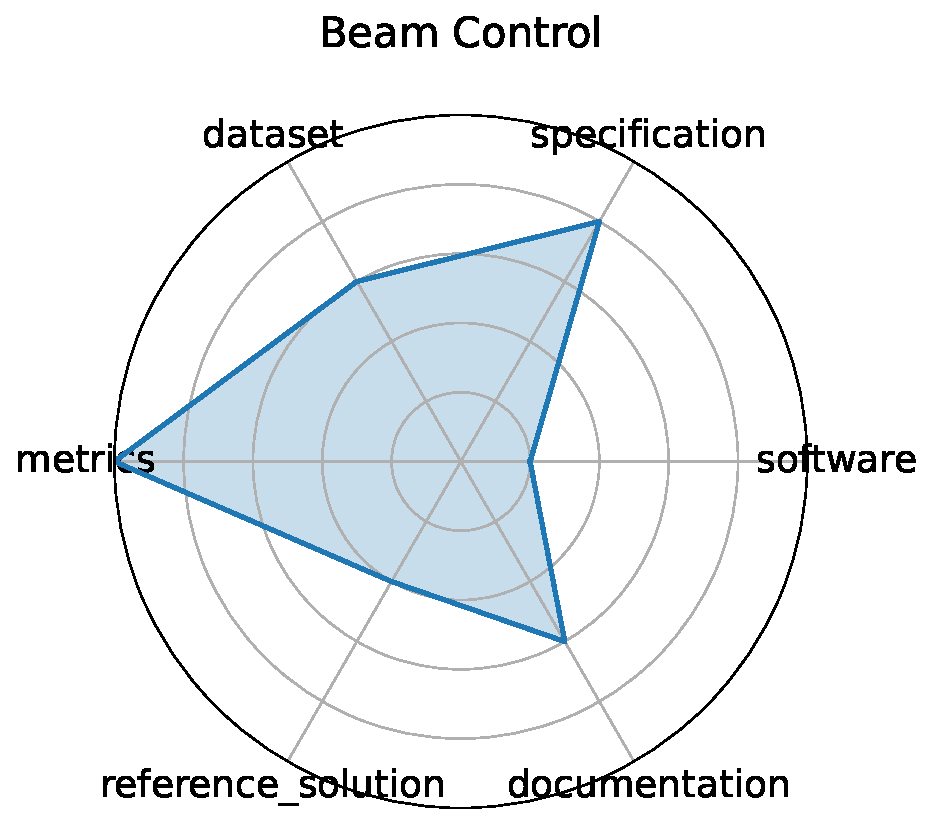
\includegraphics[width=0.2\textwidth]{beam_control_radar.pdf}
}}
\clearpage